\chapter {Methodology}

\section{Model Development Steps}
\begin{enumerate}
    \item Conduct a comprehensive analysis of existing models for PoW and PoS blockchains. Select a state-of-the-art model that employs a bottom-up approach, making it easier to incorporate new factors into it \cite{CambridgeCBECI}. Provide a comprehensive explanation of its components.

    \item Acquire a deep understanding of the interplay of microscopic factors and their macroscopic effects in Ethereum PoS \cite{MarionAnModelling}. With this knowledge, consider the limited 'post-merge' data available and identify 2-3 factors that can be integrated into the base model.

    \item Analyse data and literature relating these factors to electricity consumption in various contexts. Adhering to the principles of Rule-Based Mathematical Modelling outlined in \sref{MathematicalModellingLitRev}, develop equations related to PoS Ethereum, either by adapting existing equations to the given context or through modelling observed behaviours.

    \item Incorporate these equations into the base model. Estimate the network shares of users employing different hardware, client, and node configurations, and assign weights to different parts of the equation where possible \cite{CCRI:Institute}.

    \item Determine the contemporary metrics (e.g., gas fees, transaction count, etc.) required to implement the model proposed along with competing models. Implement all models using the same metrics to produce easily comparable values (like energy consumption per transaction) to facilitate the evaluation of the model's results \cite{CryptoCarbonRatingsInstitute2022TheNetwork}.

\end{enumerate}

\section {Evaluation Metrics}

\subsection{Quantitative}
\label{MethoologyErrorQuant}
The aim of a validation metric is to be able to assess the predictive capability of a mathematical model \cite{Kat2012ValidationError}. Results for comparison will be obtained by implementing other similar mathematical models found in the literature. Most relative-error measures compare true observed values to prediction results. However, since all models estimate the energy consumption of Ethereum, there is no true value. Thus, selecting an appropriate quantitative error measure is challenging. 

The magnitude error, which compares the relative orders of magnitude between two functions, could be used as a means of validating the results obtained. To calculate the magnitude error using \eref{eqn:ErrorMeasureEqn}, results from an experimental model with scientific data will be treated as the true value, $\boldsymbol{\mathrm{m}}$, while estimates from our 'Model-A' will replace prediction value, $\boldsymbol{\mathrm{p}}$ \cite{RussellErrorMeasure}. The suggested upper bound for a result being acceptable is $\boldsymbol{\epsilon_\mathrm{rme} \leq 0.2}$.

\begin{align}
\label{eqn:ErrorMeasureEqn}
    &\boldsymbol{\epsilon_\mathrm{rme} = \mathrm{sign(rme)} * \log_{10} (1 + |\mathrm{rme}|)}
    &\boldsymbol{ \mathrm{rme} = \mathrm{\frac{\mathrm{\sum\limits_{i=1}^{N} p_{i}^{2}} - \mathrm{\sum\limits_{i=1}^{N} m_{i}^{2}}}{\sqrt{\mathrm{\sum\limits_{i=1}^{N} p_{i}^{2}} * \mathrm{\sum\limits_{i=1}^{N} m_{i}^{2}}}}}}
\end{align}

% --------------------------------------------------------------------
\subsection{Qualitative}
\label{QualModelEvalMEthodology}
 It would be a near-impossible task to successfully verify the model through h simulate PoS Ethereum without losing its microscopic characteristics that this study relies on to improve upon the base model. Some qualitative techniques that can instead be used to verify the model include the following \cite{Al-Aomar2015ModelTechniques}:

\textbf{1. Thorough Examination of Model Inputs - } During development, the input values for each part of the model will be obtained only from scientific sources. If infeasible, anecdotal data from multiple sources must be averaged as a substitute. A 'valid' input is defined as being:
\begin{enumerate}
    \item Correct
    \item Relevant to the real-world system being modelled
    \item Being used in the model similar to the way they would be used by the real-world system being modelled
\end{enumerate}  

\textbf{2. Detailed Documentation of Model Logic - }
Every decision made during the formulation of the model must be clearly documented and well-justified using observed data or domain-specific knowledge. All assumptions will be highlighted using bold formatting.


\textbf{3. Thorough Examination of Model Outputs - }
The model's results must lie in a 'reasonable' range when compared to competing model's results \cite{Al-Aomar2015ModelTechniques}. Any discrepancies between Model-A and other models must be clearly addressed in the discussion section.   

\section {Data Gathering}

The primary scientific data source in this field is from the CCRI study \cite{CryptoCarbonRatingsInstitute2022TheNetwork}, which has been referenced in most other studies in this emerging area of research \cite{IbanezTheExpansion}. In addition to this data, a variety of sources, including blockchain crawlers for obtaining metrics such as transaction counts, and anecdotal or non-scientific sources like Reddit and Discord communities (where reputed users share their measurements), were collected and averaged. See Appendix A.

The CCRI \cite{Ccri-apiOverview} and Etherscan \cite{EtherscanProvider} APIs will be used to pursue a data-driven approach to modelling. The majority of indices publicly accessible on the CCRI website display annualized values for daily estimates. These values will be divided by 365 to acquire accurate daily figures.

% \section {Modelling The Energy Consumption Using Domain Knowledge}

% *Define everything in your modelling world, what your definition of everything is

% We care about the power coming from the grid. The AC 'At-Wall'. We gather estimations for the recommended configuration of hardware for Ethereum nodes running validator clients. 

% Also decide on which way of data gathering is better. Prepare a table of online users claiming their power consumption. Also, estimate the power consumption of the recommended configuration of hardware through manufacturer websites. This is then compared to the data from the \cite{CryptoCarbonRatingsInstitute2022TheNetwork} report actually running a single validator node to check if this bottom-up hardware estimation approach is valid. 

% Knowing the fact that increasing the number of validator clients on a single machine increases the power consumption logarithmically, we apply this assumption to the CCRI equation. We also need to account for power inefficiency of the computer by adding a factor to this equation. The report does not mention the power supply or mainboard used.

% Also need to add the syncing energy into the equation as it is not a short process. Need to model this, depending on the data and add it to the equation. (possibly for every combination of CL and EL client)
% ------------------------------------------------------------------

\section {Project Management}

Agile project management practices were employed during the course of this project. 

\subsection{Task Management}

Given the frequent topic changes throughout the project, adopting an agile methodology was critical to the success of this project. Todoist, a task management tool, was utilised for micro-task management. Its visual task board enables task categorisation by importance level, date, and macro-tasks, as demonstrated in Appendix E. Various self-set milestones were dated into my task list and, when complete, updated into my Gantt chart.

Macro-level task management was accomplished through implementing a Gantt chart. These tasks underwent drastic changes monthly due to the newfound knowledge of the research area and progress in the technical section. The latest Gantt chart is shown in \fref{Figure:ganttUpdated}, with the original version in Appendix G. 

\subsection{Time Management}

The Gantt chart also facilitated macro-level time management by allocating time for each major project task across both semesters. Realistic allocations were made and updated monthly, accounting for other coursework and unexpected delays. 

Furthermore, brief summaries of relevant literature papers read during the course of this project were recorded in a Word document (Appendix F). This approach allowed for the efficient organisation of ideas and prevented rereading papers, saving time. 


\begin{figure}[!htb]
    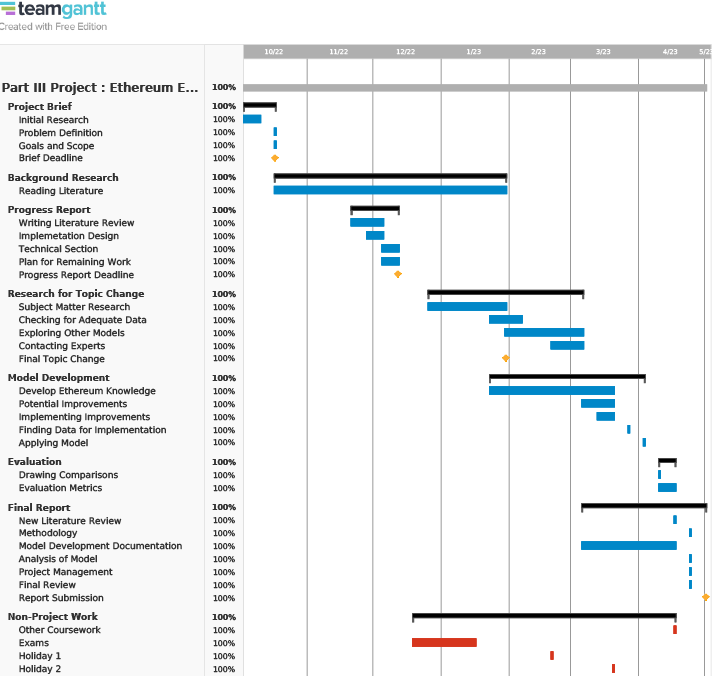
\includegraphics[width=14cm,center]{Figures/ganttUpdated.png}
    \caption{Latest version of the Gantt Chart. An older version of the Gantt Chart}
    \label{Figure:ganttUpdated}
\end{figure}



\subsection{Risk Management}

Forseen risks associated with taking on such a novel project have been compiled into \tref{Figure:RiskTable}, ordered by descending risk score, calculated as the quotient of $\mathrm{Probability * Impact}$.

\begin{table}[!htb]
    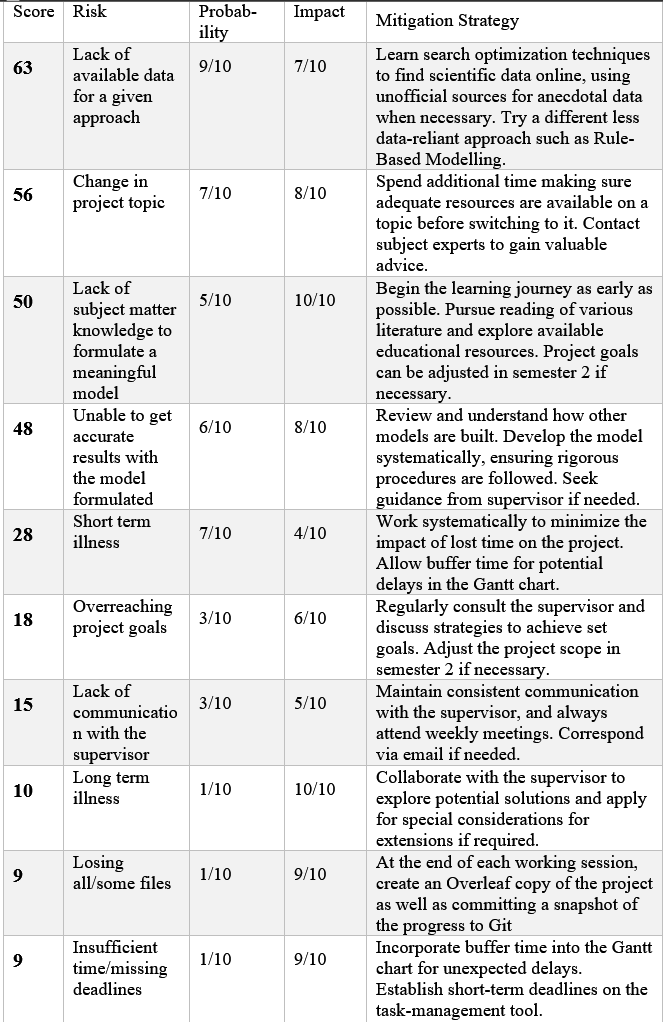
\includegraphics[width=14cm,center]{Figures/RiskTable2.png}
    \caption{Risk Analysis table taken from the progress report submission.}
    \label{Figure:RiskTable}
\end{table}